\documentclass[12pt]{article}

\addtolength{\oddsidemargin}{-.875in}
\addtolength{\evensidemargin}{-.875in}
\addtolength{\textwidth}{1.75in}

\addtolength{\topmargin}{-.875in}
\addtolength{\textheight}{1.75in}

\openup 1em

%macro for commenting
\usepackage{color}
\newcommand{\leo}[1]{{\color{blue}{\it leo: #1}}}
\newcommand{\xbeta}{\boldsymbol X_i^T \boldsymbol\beta}


\usepackage[round]{natbib}

\usepackage{rotating}
\usepackage{graphicx}
\usepackage{subcaption}

\usepackage{float}

\usepackage{amsthm,amsmath} 
\usepackage{amssymb}
\usepackage{subcaption}
\captionsetup{compatibility=false}

\usepackage[utf8]{inputenc}
%\usepackage{algorithm}
%\usepackage[noend]{algpseudocode}
\usepackage[]{algorithm2e}


\newtheorem{theorem}{Theorem}
\newtheorem{corollary}{Corollary}


\usepackage{mhequ}
\newcommand{\be}{\begin{equs}}
\newcommand{\ee}{\end{equs}}
\newcommand{\bfi}{\begin{figure}[H]}
\newcommand{\efi}{\end{figure}}
\newcommand{\bsfi}{\begin{subfigure}[t]}
\newcommand{\esfi}{\end{subfigure}}
\newcommand{\bb}[1]{\mathbb{#1}}
\newcommand{\mc}[1]{\mathcal{#1}}
\newcommand{\bl}{\boldsymbol}
\newcommand{\X}{\boldsymbol X}
\newcommand{\Y}{\boldsymbol Y}
\newcommand{\Z}{\boldsymbol Z}
\newcommand{\W}{\boldsymbol W}
\newcommand{\I}{\boldsymbol I}
\newcommand{\V}{\boldsymbol V}
\newcommand{\bmu}{\boldsymbol \mu}
\newcommand{\bSigma}{\boldsymbol \Sigma}
\newcommand{\E}{\bb E}




\thispagestyle{empty}
\baselineskip=28pt

\title
    {Random-Factor Tensor Factorization \\for Removing Batch Effects in Graphs}



%\author{
%     Leo L. Duan and
%     Joshua T. Vogelstein
%    % \textsuperscript{*}\footnotemark[2]\and
%}


\date{}
\begin{document}


\section{Data exploration}

The reason for large misclassification error?
\bfi
\centering
\bsfi{0.5\columnwidth}
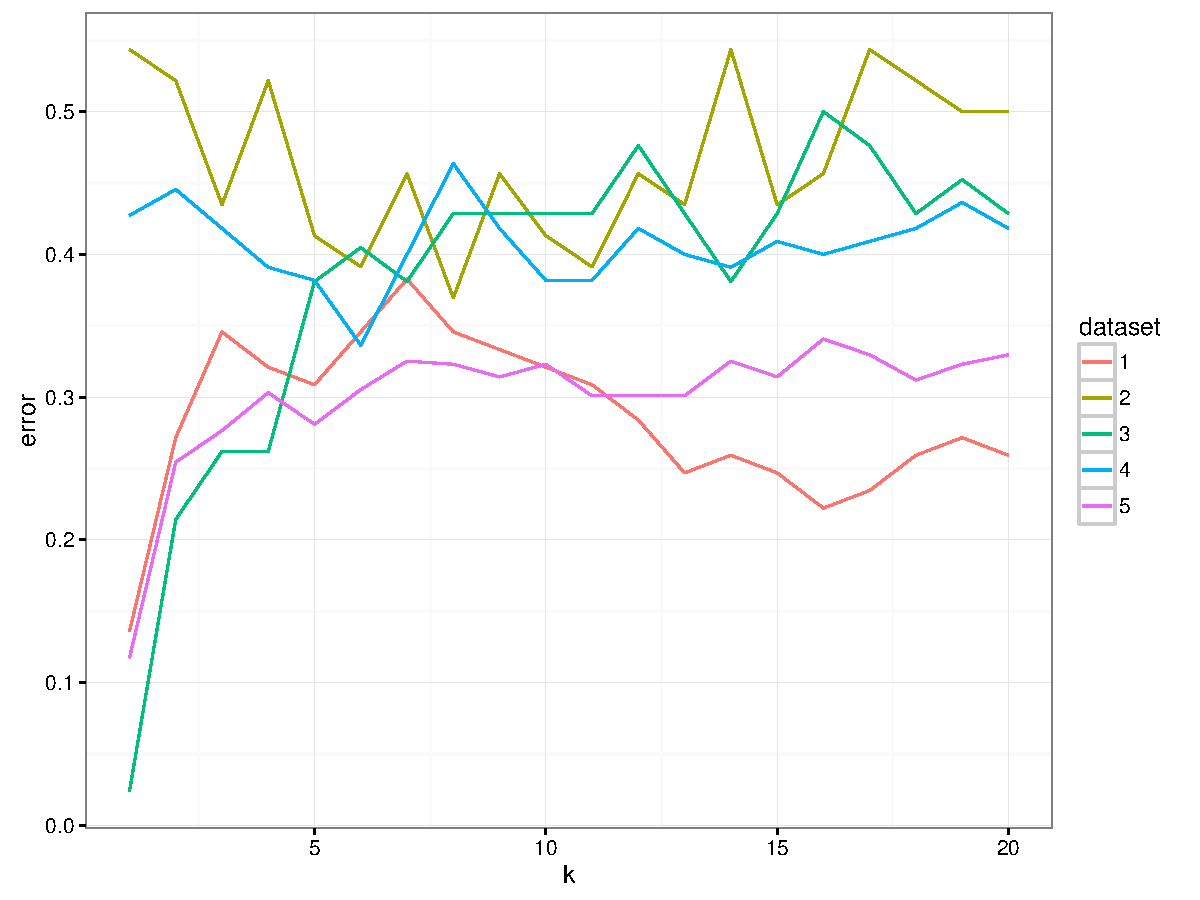
\includegraphics[width=1\columnwidth]{../BatchEffectRemoval/sex_classification_raw_5dataset}
\esfi
\caption{Classification error using directly the adjacency matrices. Datasets with sex are heterogeneous: 2 have very weak signal, while 3 have good signal.}
\efi

For good data (taking 1,3,5 above and renumber), the classification with all subjects together doesn't seem to generate problem. 


\bfi
\centering
\bsfi{0.5\columnwidth}
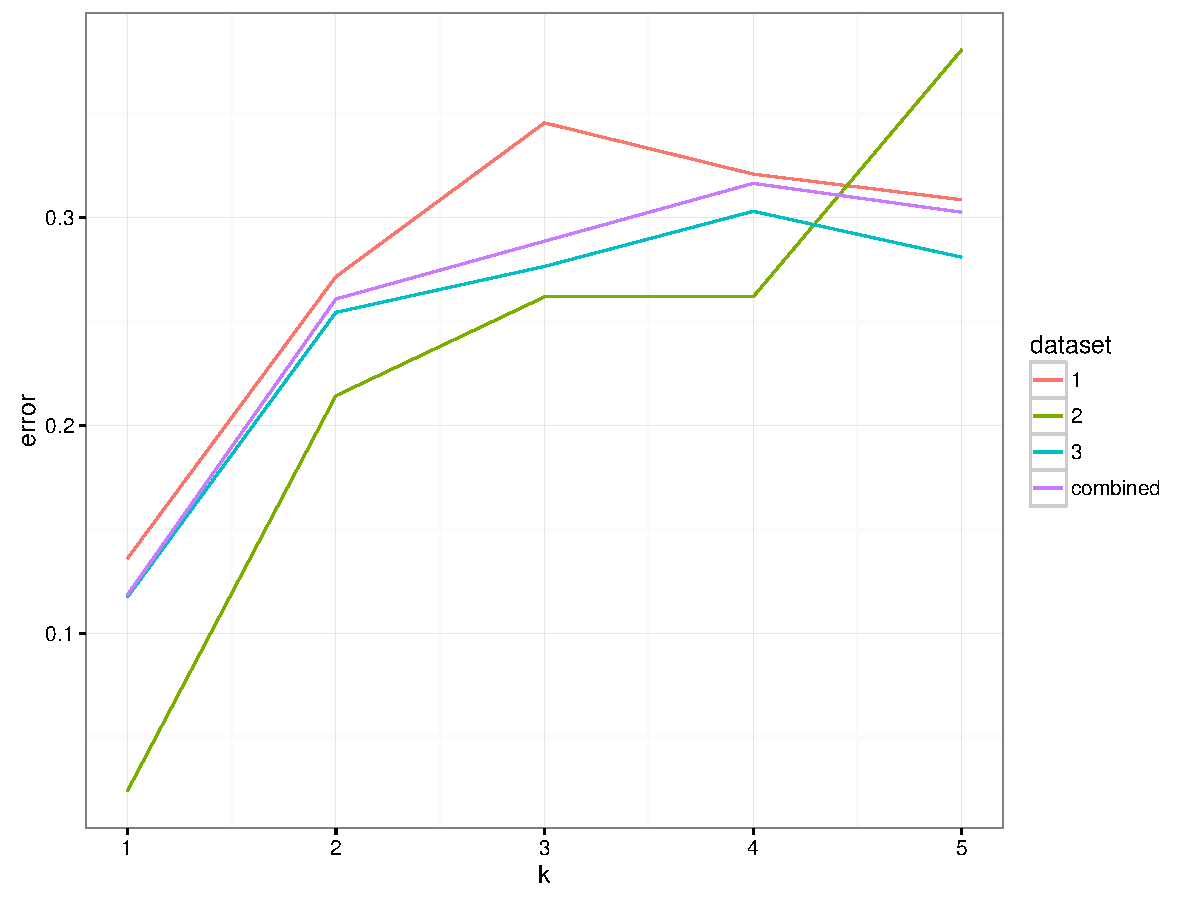
\includegraphics[width=1\columnwidth]{../BatchEffectRemoval/selection_dataset_good.pdf}
\esfi
\caption{Combining the 3 datasets with strong signal and do joint classifcation, yielding relatively satisfactory performance}
\efi

\section{Joint Diagonalization}

Consider joint diagonalization as a dimension reduction tool, assess its classification performance with the reduced vector in each dataset.

When the sample size is small (batch 1: 81 and batch 2 42), random factor model has performance close to the raw adjacency matrix; the shared factor performs worse. 

But when the sample size is large (batch 3: 452), both factor models perform worse.

\bfi
\centering
\bsfi{1\columnwidth}
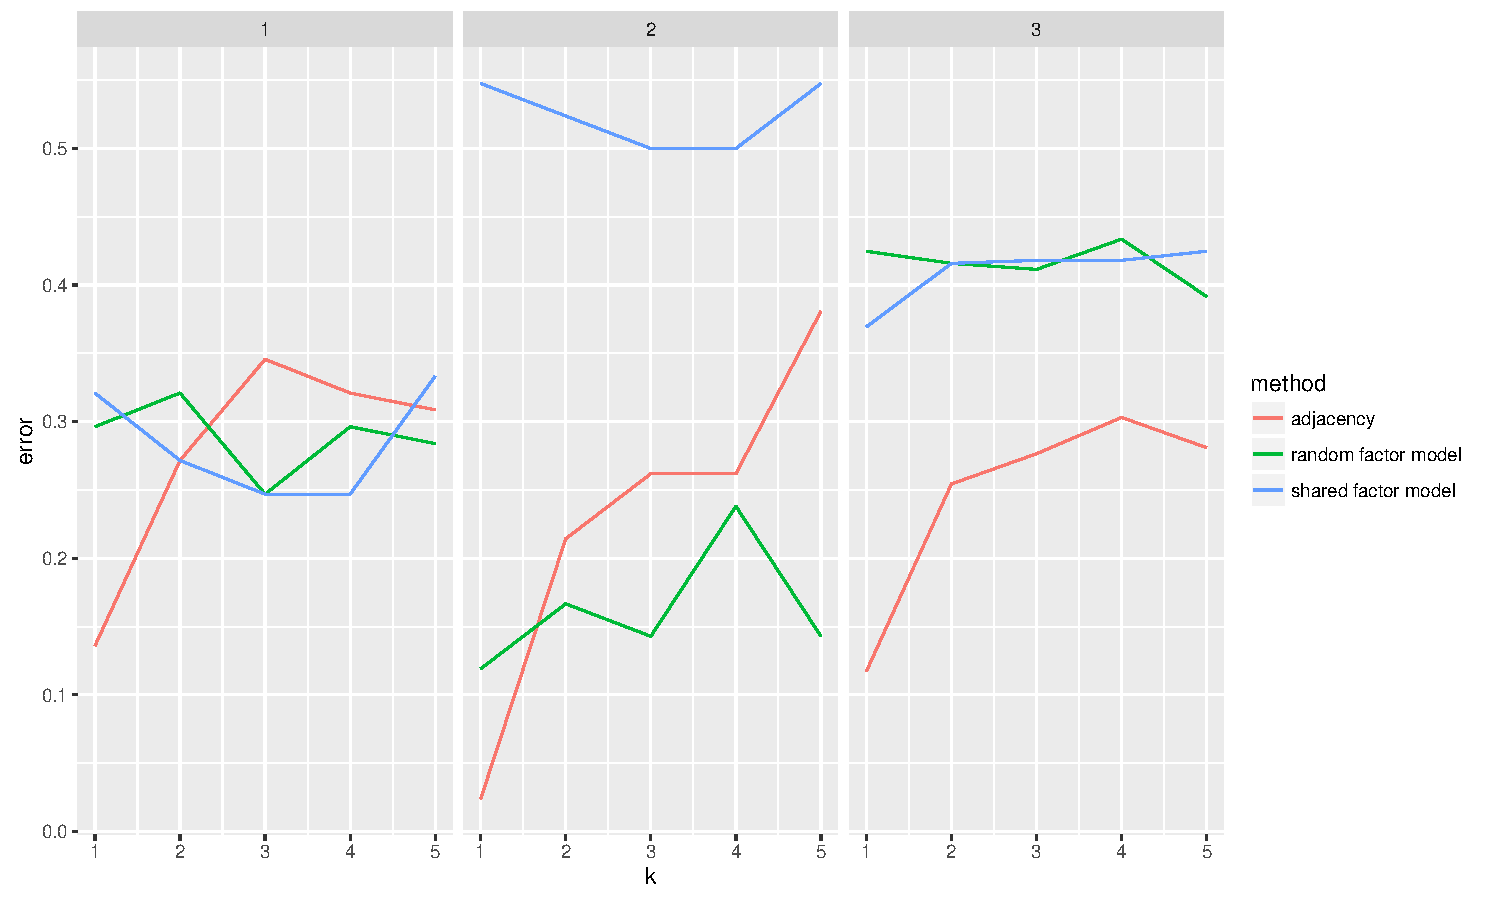
\includegraphics[width=1\columnwidth]{../BatchEffectRemoval/knnErrorPerDataset}
\esfi
\caption{Classification error in 3 datasets}
\efi

Combining together, the classification error is close the ones in dataset 3.


\bfi
\centering
\bsfi{1\columnwidth}
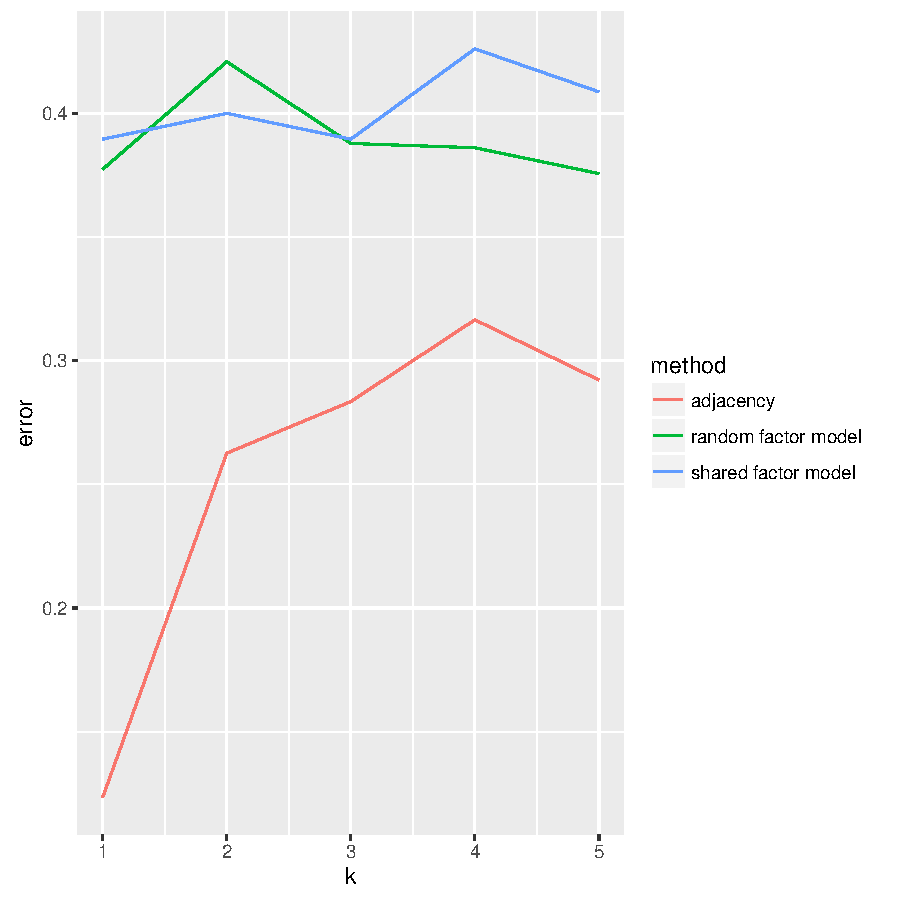
\includegraphics[width=.5\columnwidth]{../BatchEffectRemoval/knnErrorCombined}
\esfi
\caption{Classification error in 3 datasets}
\efi

This is likely due to the heterogenity inside dataset 3, huge variance can be seen in dataset 3.

\bfi
\centering
\bsfi{1\columnwidth}
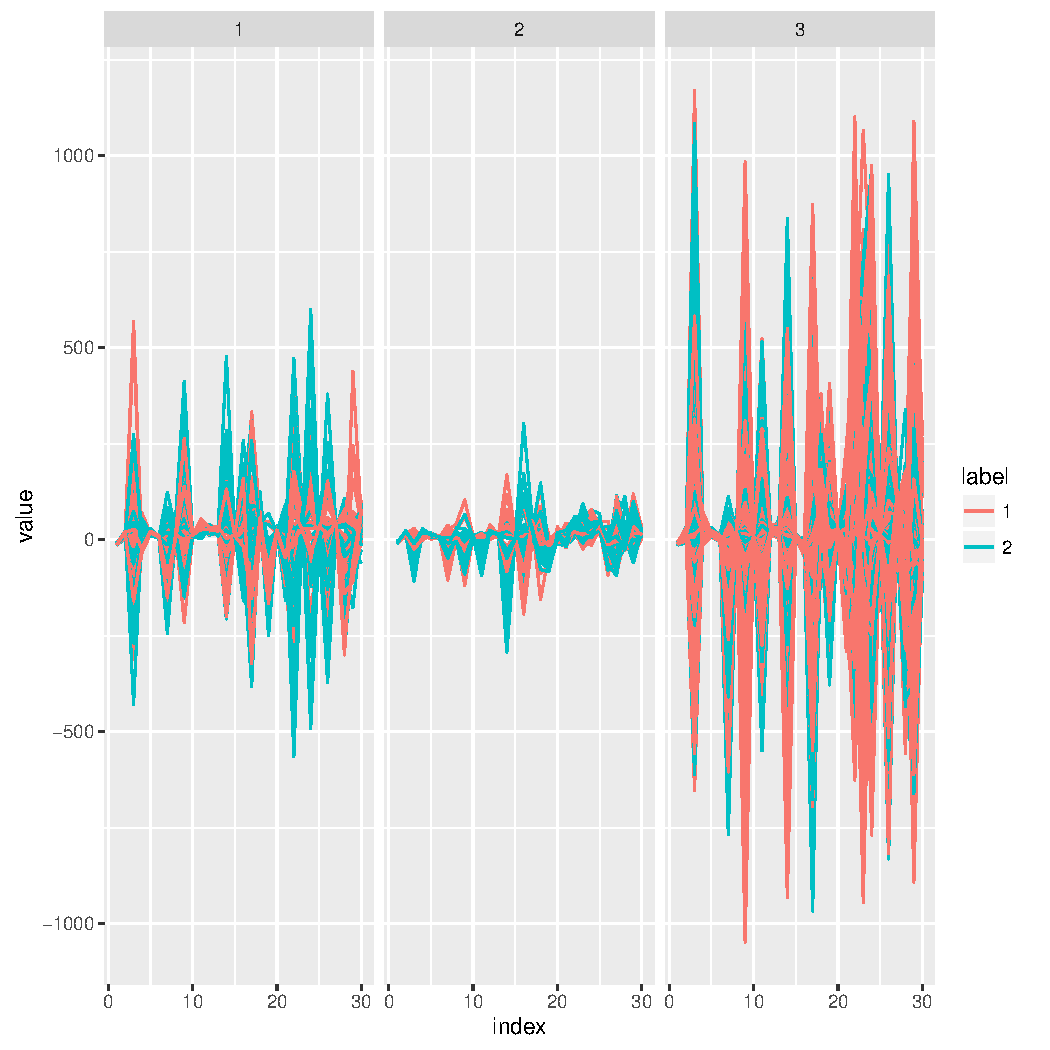
\includegraphics[width=.5\columnwidth]{../BatchEffectRemoval/core}
\esfi
\caption{Core estimate in 3 datasets}
\efi

\section{Batch effect removal}


\bfi
\centering
\bsfi{1\columnwidth}
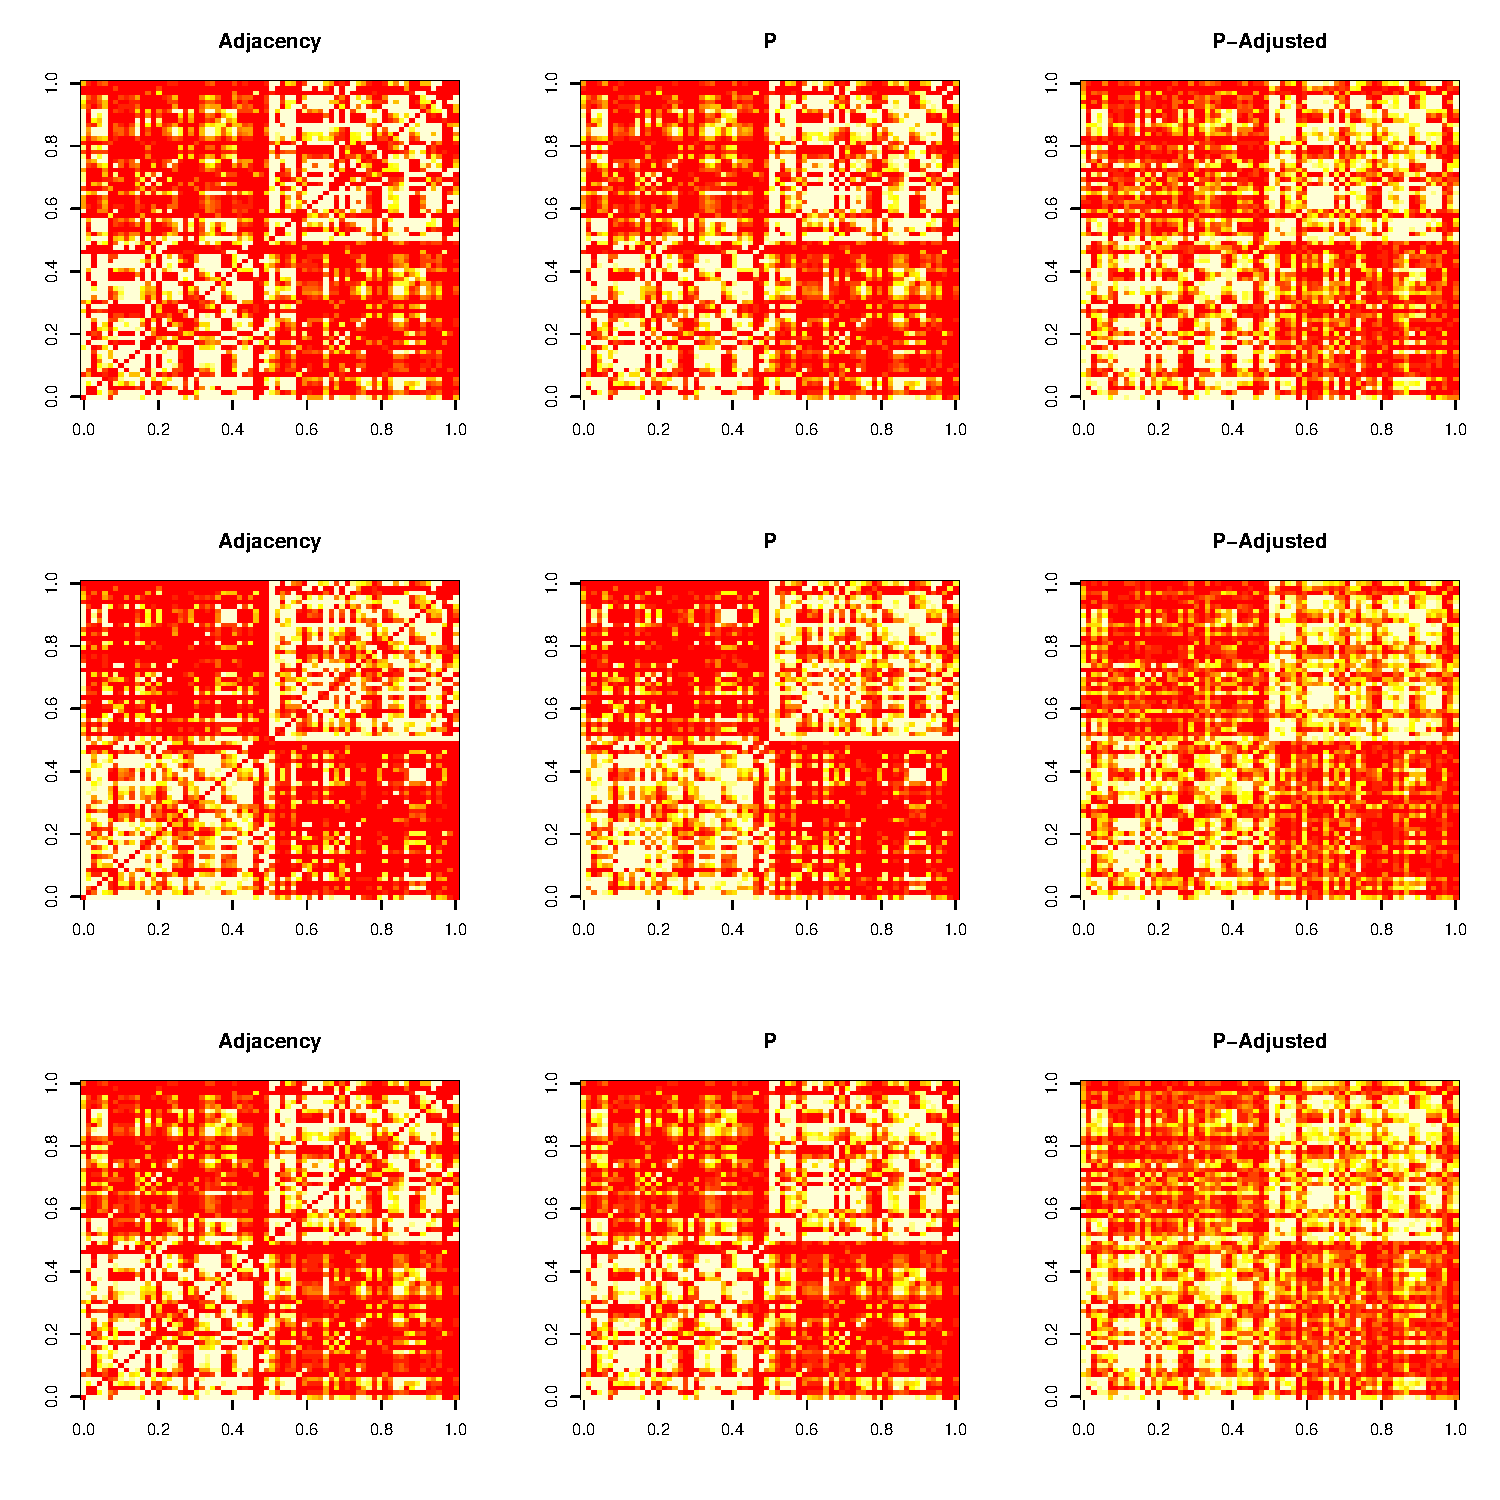
\includegraphics[width=1\columnwidth]{../BatchEffectRemoval/fitted_dataset.pdf}
\esfi
\caption{Avg Est}
\efi


\bfi
\centering
\bsfi{1\columnwidth}
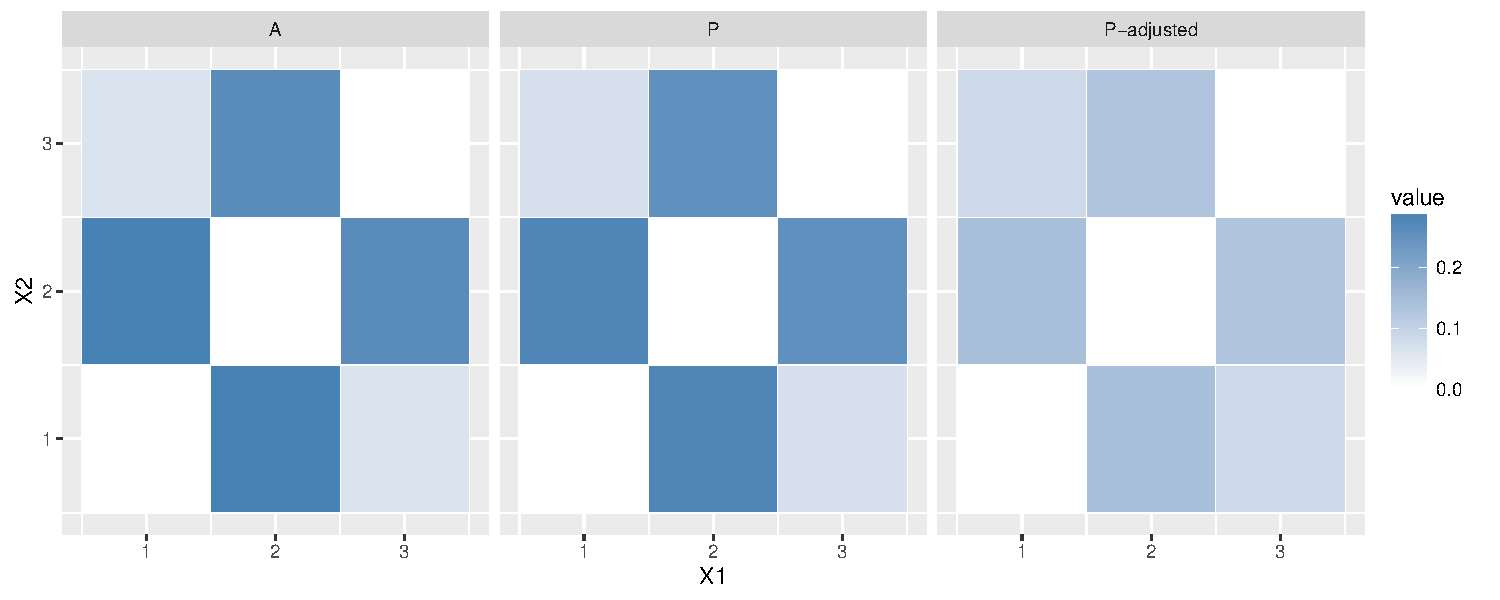
\includegraphics[width=1\columnwidth]{../BatchEffectRemoval/distance_between_dataset}
\esfi
\caption{Avg Est}
\efi

\section{Next?}

1. The rank is currently too high. To reduce variance, use a full rank average matrix first in each batch.

$$ \text{logit}^{-1}(P_{ji})  = Z_j + F_j C_{ji} F_j^T$$

2. Breaking the large dataset into smaller sets and applying the model.

3. Non-parametric method on $F_j$ if the above doesn't help much.



\end{document}
